\documentclass[8pt]{beamer}
% \beamertemplateshadingbackground{brown!70}{yellow!10}
\mode<presentation>
{
  %\usetheme{Warsaw}
  \usecolortheme{crane}
  % or ...

  % \setbeamercovered{transparent}
  % \setbeamercovered{
  %   still covered={\opaqueness<1>{50}\opaqueness<2->{20}}
  % }
%    \setbeamercovered{invisible}
  % or whatever (possibly just delete it)
}
\setbeamertemplate{navigation symbols}{}
% \setbeamertemplate{footline}[frame number]{}
\usepackage{tikz,pgfplots}
\pgfplotsset{compat=newest}
\usepackage[utf8]{inputenc}
\usetikzlibrary{patterns}
\usepackage{amssymb}
\usepackage{amsmath}
\usepackage{colortbl}
%\usepackage{multicol}
\usepackage{cancel}
\usepackage{ulem}
\usepackage{multirow}
\usepackage{relsize}
\usepackage{algorithm}
\usepackage{algorithmic}
\usepackage{forloop}% http://ctan.org/pkg/forloop
\newcounter{loopcntr}
\newcommand{\rpt}[2][1]{%
  \forloop{loopcntr}{0}{\value{loopcntr}<#1}{#2}%
}
%\pagestyle{plain}
%\input{defs2}
\def\opt{{\textsc{OPT}_k}}
\def\const{{\mathrm{const}}}
\def\nnz{{\mathrm{nnz}}}
\def\r{\sfrac{\sigma_{\w}^2}{\sigma_{\xib}^2}}
\def\rm{\sfrac{\sigma_{\xib}^2}{\sigma_{\w}^2}}
\def\cmark{\Green{\checkmark}}
\def\xmark{\Red{\large\sffamily x}}
\newcommand{\pdet}{{\mathrm{pdet}}}
\newcommand{\MSPE}[1] {{\mathrm{MSPE}\big[#1\big]}}
\newcommand{\MSE}[1] {{\mathrm{MSE}\big[#1\big]}}
\def\Poisson{{\operatorname{Poisson}}}
\def\PB{{\operatorname{PB}}}
\newcommand{\DP}[1]{\mathcal{DP}^{#1}}
\def\Ic{\mathcal{I}}
\def\Jc{\mathcal{J}}
\def\Mc{\mathcal M}
\def\Ec{\mathcal E}
\def\sr{{\mathrm{sr}}}
\def\ktd{{k^{\underline{d}}}}
\def\Det{{\mathrm{Det}}}
\def\detu{{\widecheck{\mathrm{Det}}_\mu^\gamma}}
\def\deto{{\widehat{\mathrm{Det}}_\mu^\gamma}}
\def\Zu{{\widecheck{Z}_\mu^{\gamma}}}
\def\Zo{{\widehat{Z}_\mu^{\gamma}}}
\def\Zun{{\widecheck{Z}_\mu^{\gamma_n}}}
\def\Zon{{\widehat{Z}_\mu^{\gamma_n}}}
\newcommand{\Er}{\mathrm{Er}}
\newif\ifDRAFT
\DRAFTtrue
\ifDRAFT
\newcommand{\marrow}{\marginpar[\hfill$\longrightarrow$]{$\longleftarrow$}}
\newcommand{\niceremark}[3]
   {\textcolor{red}{\textsc{#1 #2:} \marrow\textsf{#3}}}
\newcommand{\ken}[2][says]{\niceremark{Ken}{#1}{#2}}
\newcommand{\manfred}[2][says]{\niceremark{Manfred}{#1}{#2}}
\newcommand{\michael}[2][says]{\niceremark{Michael}{#1}{#2}}
\newcommand{\michal}[2][says]{\niceremark{Michal}{#1}{#2}}
\newcommand{\feynman}[2][says]{\niceremark{Feynman}{#1}{#2}}
%\usepackage[inline]{showlabels}
\else
\newcommand{\ken}[1]{}
\newcommand{\michael}[1]{}
\newcommand{\michal}[1]{}
\newcommand{\feynman}[1]{}
\fi
\newcommand{\norm}[1]{{\| #1 \|}}

\newcommand{\deff}{d_{\textnormal{eff}}}
\def\ee{\mathrm{e}}
\newcommand\mydots{\makebox[1em][c]{.\hfil.\hfil.}}
\def\Sd{\mathscr{S}_{\!d}}
\newcommand{\dx}{\dxy_{\!\cal X}}
\newcommand{\dxk}{\dxy_{\!\cal X}^k}
\newcommand{\dk}{\dxy^k}
\newcommand{\dxy}{\mathrm{D}}
\def\simiid{\overset{\textnormal{\fontsize{6}{6}\selectfont
i.i.d.}}{\sim}}
%\newcommand{\Dxy}{D_{\!\cal X\!,\cal Y}}
\def\vskx{{\mathrm{VS}_{\!\dx}^k}}
\def\vsk{{\mathrm{VS}_{\!D}^k}}
\def\vskxm{{\mathrm{VS}_{\!\dx}^{k-1}}}
\def\vskm{{\mathrm{VS}_{\!D}^{k-1}}}
\def\vsdx{{\mathrm{VS}_{\!\dx}^d}}
\def\vsd{{\mathrm{VS}_{\!D}^d}}
\newcommand{\vs}[1]{{\mathrm{VS}_{\!D}^{#1}}}
\newcommand{\sigd}{\boldsymbol\Sigma_{\!\dx}}
\def\wols{\w_{\mathrm{LS}}}
\def\wds{\boldsymbol\w_{\!D}^*}
\def\kd{K_{\!\dx}}

\def\poly{{\mathrm{poly}}}
\def\polylog{{\mathrm{polylog}}}
\def\DPP{{\mathrm{DPP}}}
\def\DPPcor{{\DPP_{\!\mathrm{cor}}}}
\def\DPPens{{\DPP_{\!\mathrm{ens}}}}
\newcommand{\DPPreg}[1]{{\DPP_{\!\mathrm{reg}}^{#1}}}
\def\Vol{{\mathrm{VS}}}
\def\Lev{{\mathrm{Lev}}}
\newcommand\todod[1]{\Red{\# DH: #1}}
\newcommand{\explain}[2]{\mathrel{\overset{\makebox[0pt]{\text{\tiny
#1}}}{#2}}}
\def\tot {{\mathrm{tot}}}
\def\checkmark{\tikz\fill[scale=0.4](0,.35) -- (.25,0) --
(1,.7) -- (.25,.15) -- cycle;}
\newcommand{\mnote}[1]{{\bf\large \Magenta{*}}\marginpar{\small \Magenta{#1}}}
\newcommand{\bnote}[1]{{\bf #1}}

\newcommand{\sqrtshort}[1]{{\sqrt{\white{\Big|}\!\!\smash{\text{\fontsize{9}{9}\selectfont$#1$}}}}}
\newenvironment{proofof}[2]{\par\vspace{2mm}\noindent\textbf{Proof of {#1} {#2}}\ }{\hfill\BlackBox}
\newcommand{\sets}[2]
{{\hspace{-0.3mm}[\hspace{-0.3mm}#1\hspace{-0.3mm}]\hspace{-0.3mm}\choose
\hspace{-0.3mm}#2\hspace{-0.3mm}}}
\DeclareMathOperator{\sgn}{\textnormal{sgn}}
\DeclareMathOperator{\adj}{\textnormal{adj}}
\def\Rb{{\mathbf{R}}}
\DeclareMathOperator{\ws}{\widetilde{\w}}
\newcommand{\inote}[1]{{\bf {#1}}}
\def\xib{\boldsymbol\xi}
\def\Sigmab{\mathbf{\Sigma}}
\def\Sigmabh{\widehat{\Sigmab}}
\def\Sigmabt{\widetilde{\Sigmab}}
\def\S{\mathbf{S}}
\def\T{\mathbf{T}}
\def\xt{\tilde{x}}
\def\xbt{\widetilde{\x}}
\def\xbh{\widehat{\x}}
\def\ubh{\widehat{\u}}
\def\dom {{\mathrm{dom}}}
\def\val {{\mathrm{val}}}
\def\out {{\mathrm{out}}}
\def\iin  {{\mathrm{iin}}}
\def\s {\mathbf{s}}
\def\q {\mathbf{q}}
\def\qt{\tilde{q}}
\def\itld {j}
\def\ubt {\tilde{\u}}
\def\n{\{1..n\}}
\def\cb {\mathbf{c}}
\def\cW{\mathcal W}
\def\Xt{\widetilde{X}}
\def\Dbt{\widetilde{\D}}
\def\xtb{\tilde{\mathbf{x}}}
\def\ytb{\tilde{\mathbf{y}}}
\def\Xtb{\widetilde{\mathbf{X}}}
\def\Xbb{\overline{\X}}
\def\Xb{{\bar{\X}}}
\def\ybb{\overline{\y}}
\def\f{{\mathbf{f}}}
\def\g{{\mathbf{g}}}
\def\fbb{{\overline{\f}}}
\def\fb{{\overline{f}}}
\def\Xc{\mathcal{X}}
\def\W{\mathbf W}
\def\L{\mathbf{L}}
\def\Rb{\mathbf R}
\def\Pc{\mathcal{P}}
\def\Nc{\mathcal{N}}
\def\Pt{\widetilde{P}}
\def\Hc{\mathcal{H}}
\def\Wc{\mathcal{W}}
\def\Cc{\mathcal{C}}
\def\p{\mathbf p}
%\def\r{\mathbf r}
\def\Y{\mathbf Y}
\def\H{\mathbf H}
\def\K{\mathbf K}
\def\Kh{\widehat{K}}
\def\Kbh{{\widehat{\K}}}
\def\Q{\mathbf Q}
\def\Qbar{{\bar{\mathbf Q}}}
\def\Ytb{\widetilde{\mathbf{Y}}}
\def\c{{n-d\choose s-d}}
\DeclareMathOperator{\Proj}{Proj}
\newcommand{\Span}{\mathrm{span}}
\newcommand{\ofsubt}[1]{\mbox{\scriptsize \raisebox{0.25pt}{$(#1)$}}}
%\raisebox{0.5pt}{$($}}#1\mbox{\tiny \raisebox{0.5pt}{$)$}}}
\newcommand{\ofsub}[1]{\mbox{\small \raisebox{0.0pt}{$(#1)$}}}
%\newcommand{\ofsubb}[1]{\mbox{\footnotesize \raisebox{0.5pt}{$(#1)$}}}
%\newcommand{\ofsub}[1]{(#1)}
%\newcommand{\ofsub}[1]{\mbox{\tiny$|$\hspace{-0.5pt}\raisebox{-0.5pt}{$#1$}}}
\newcommand{\of}[2]{{#1{\!\ofsub{#2}}}}
\newcommand{\oft}[2]{{#1{\!\ofsubt{#2}}}}
\newcommand{\fof}[2]{{#1({#2})}}
\newcommand{\yof}[2]{{#1{\ofsub{#2}}}}
%\newcommand{\yofb}[2]{{#1{\ofsubb{#2}}}}
\newcommand{\lazy}{FastRegVol}
\newcommand{\volsamp}{RegVol}

\newcommand{\Sm}{{S_{-i}}}
\newcommand{\Sp}{{S_{+i}}}
\ifx\BlackBox\undefined
\newcommand{\BlackBox}{\rule{1.5ex}{1.5ex}}  % end of proof
\fi
%\renewcommand{\dagger}{+}
\DeclareMathOperator*{\argmin}{\mathop{\mathrm{argmin}}}
\DeclareMathOperator*{\argmax}{\mathop{\mathrm{argmax}}}
\DeclareMathOperator*{\diag}{\mathop{\mathrm{diag}}}
\def\x{\mathbf x}
\def\y{\mathbf y}
\def\ybh{\widehat{\mathbf y}}
\def\ybb{\bar{\mathbf y}}
\def\xbb{\bar{\mathbf x}}
\def\yb{{\bar y}}
\def\ybt{\widetilde{\mathbf y}}
\def\yh{\widehat{y}}
\def\yhb{\widehat{\y}}
\def\yt{\widetilde{y}}
\def\z{\mathbf z}
\def\a{\mathbf a}
\def\b{\mathbf b}
\def\w{\mathbf w}
\def\v{\mathbf v}
\def\m{\mathbf m}
\def\wbh{\widehat{\mathbf w}}
\def\wh{\widehat{\mathbf w}}
\def\vbh{\widehat{\mathbf v}}
\def\wbt{\widetilde{\mathbf w}}
\def\e{\mathbf e}
\def\zero{\mathbf 0}
\def\one{\mathbf 1}
\def\u{\mathbf u}
\def\ubbar{\bar{\mathbf u}}
\def\f{\mathbf f}
\def\ellb{\boldsymbol\ell}

\def\X{\mathbf X}
\def\Xs{\widetilde{\X}}
\def\B{\mathbf B}
\def\A{\mathbf A}
\def\C{\mathbf C}
\def\U{\mathbf U}
\def\Ubt{\widetilde{\mathbf U}}
\def\Ubh{\widehat{\mathbf U}}
\def\Ubbar{\bar{\mathbf U}}
\def\F{\mathbf F}
\def\D{\mathbf D}
\def\V{\mathbf V}
\def\M{\mathbf M}
\def\Mh{\widehat{\mathbf M}}
%\def\S{\mathbf S}
\def\Stb{\widetilde{\mathbf{S}}}
\def\Sbh{\widehat{\mathbf{S}}}
\def\St{\widetilde{\S}}
\def\Sh{\widehat{S}}
\def\Sc{\mathcal{S}}
\def\Fc{\mathcal{F}}
\def\Vc{\mathcal{V}}
\def\Bc{\mathcal{B}}
\def\Dc{\mathcal{D}}
\def\Z{\mathbf Z}
\def\Zbh{\widehat{\mathbf Z}}
\def\Zbt{\widetilde{\mathbf Z}}
\def\Abh{\widehat{\mathbf A}}
\def\I{\mathbf I}
\def\Ic{\mathcal I}
\def\II{\mathbf {I \!\,I}}
%\def\II{\boldsymbol {\mathbb I}}
\def\A{\mathbf A}
\def\P{\mathbf P}
\def\Ph{\widehat{\mathbf P}}
\def\cP{\mathcal P}
\def\cR{\mathcal R}
\def\Xt{\widetilde{\mathbf{X}}}
\def\Xh{\widehat{\mathbf{X}}}
\def\Rh{\widehat{R}}
\def\Ot{\widetilde{O}}
\def\At{\widetilde{\A}}


\def\E{\mathbb E}
\def\R{\mathbb R}
\def\N{\mathbb N}
\def\Pr{\mathrm{Pr}}
%\def\C{\mathbb C}
\def\tr{\mathrm{tr}}
\def\Sbar{{\bar{S}}}
\def\cS{{\mathcal{S}}}
\def\Tbar{{\bar{T}}}
\def\Tt{{\widetilde{T}}}
\def\rank{\mathrm{rank}}
\def\Prob{\mathrm{Prob}}
\def\Var{\mathrm{Var}}
\def\Xinv{(\X^\top\X)^{-1}}
\def\XinvS{(\X_S\X_S^\top)^{-1}}
\def\ABinvS{(\A_S\B_S^\top)^{-1}}
\def\ABinv{(\A\B^\top)^{-1}}
\def\xinv{\x_i^\top\Xinv\x_i}
\def\Xinvr{(\lambda\I+\X_{-1}^\top\X_{-1})^{-1}}
\def\pdet{\mathrm{pdet}}
\newcommand{\vol}{\mathrm{vol}}
%\newcommand{\defeq}{:=}
\newcommand{\defeq}{\stackrel{\textit{\tiny{def}}}{=}}
\newcommand{\di}{{[d+1]_{-i}}}
\newcommand{\cov}{\mathrm{cov}}
\let\origtop\top
\renewcommand\top{{\scriptscriptstyle{\origtop}}} % this makes transpose not so big

\definecolor{silver}{cmyk}{0,0,0,0.3}
\definecolor{yellow}{cmyk}{0,0,0.9,0.0}
\definecolor{reddishyellow}{cmyk}{0,0.22,1.0,0.0}
\definecolor{black}{cmyk}{0,0,0.0,1.0}
\definecolor{darkYellow}{cmyk}{0.2,0.4,1.0,0}
\definecolor{orange}{cmyk}{0.0,0.7,0.9,0}
\definecolor{darkSilver}{cmyk}{0,0,0,0.1}
\definecolor{grey}{cmyk}{0,0,0,0.5}
\definecolor{darkgreen}{cmyk}{0.6,0,0.8,0}
\newcommand{\Red}[1]{{\color{red}  {#1}}}
\newcommand{\Purple}[1]{{\color{purple}  {#1}}}
\newcommand{\Magenta}[1]{{\color{magenta}{#1}}}
\newcommand{\Green}[1]{{\color{darkgreen}  {#1}}}
\newcommand{\Blue}[1]{\color{blue}{#1}\color{black}}
\newcommand{\Orange}[1]{\textcolor{orange}{#1}\color{black}}
\newcommand{\Brown}[1]{{\color{brown}{#1}\color{black}}}
\newcommand{\Grey}[1]{{\color{grey}{#1}\color{black}}}
\newcommand{\white}[1]{{\textcolor{white}{#1}}}
\newcommand{\yellow}[1]{{\textcolor{reddishyellow}{#1}}}
\newcommand{\darkYellow}[1]{{\textcolor{darkYellow}{#1}}}
\newcommand{\grey}[1]{{\textcolor{grey}{#1}}}

\DeclareMathOperator{\half}{\frac{1}{2}}

\ifx\proof\undefined
\newenvironment{proof}{\par\noindent{\bf Proof\ }}{\hfill\BlackBox\\[2mm]}
\fi

\ifx\theorem\undefined
\newtheorem{theorem}{Theorem}
\fi

\ifx\example\undefined
\newtheorem{example}{Example}
\fi

\ifx\condition\undefined
\newtheorem{condition}{Condition}
\fi
\ifx\property\undefined
\newtheorem{property}{Property}
\fi

\ifx\lemma\undefined
\newtheorem{lemma}{Lemma}
\fi

\ifx\proposition\undefined
\newtheorem{proposition}{Proposition}
\fi

\ifx\remark\undefined
\newtheorem{remark}{Remark}
\fi

\ifx\corollary\undefined
\newtheorem{corollary}{Corollary}
\fi

\ifx\definition\undefined
\newtheorem{definition}{Definition}
\fi

\ifx\conjecture\undefined
\newtheorem{conjecture}{Conjecture}
\fi

\ifx\axiom\undefined
\newtheorem{axiom}{Axiom}
\fi

\ifx\claim\undefined
\newtheorem{claim}{Claim}
\fi

\ifx\assumption\undefined
\newtheorem{assumption}{Assumption}
\fi

\ifx\condition\undefined
\newtheorem{condition}{Condition}
\fi


\edef\polishl{\l}
\setlength{\columnsep}{0.7em}
\setlength{\columnseprule}{0mm}
\setlength{\arrayrulewidth}{1pt} 

\newcommand{\svr}[1]{{\textcolor{darkSilver}{#1}}}
\definecolor{brightyellow}{cmyk}{0,0,0.7,0.0}
\definecolor{lightyellow}{cmyk}{0,0,0.3,0.0}
\definecolor{lighteryellow}{cmyk}{0,0,0.1,0.0}
\definecolor{lightestyellow}{cmyk}{0,0,0.05,0.0}

%  \fboxsep=3pt
% %\fboxsep=0mm%padding thickness
% \fboxrule=2pt%border thickness


\setkeys{Gin}{width=0.7\textwidth}

\title[Surrogate design]{
  Exact expressions for double descent and implicit regularization via surrogate random design
}
\date{TOPML'21, 04-20-2021}
\author[]{Micha{\polishl } Derezi\'{n}ski, \ Feynman Liang,
  \ Michael Mahoney\\UC Berkeley}

\begin{document}

\begin{frame}
  \maketitle
\end{frame}

\begin{frame}
  \frametitle{Simple model of double descent}

  {\centering
    ``Classical'' ML: \qquad\textit{parameters} $\ll$ \textit{data}\quad~\\
    ``Modern'' ML
    % \footnote{Hastie, Montanari, Rosset, Tibshirani (2019).~arXiv:1903.08560}
    % \footnote{Bartlett, Long, Lugosi, Tsigler (2019).~arXiv:1906.11300}
    : \qquad\textit{parameters} $\gg$ \textit{data}\quad~\\
    \textit{Phase transition}: \qquad\textit{parameters} $\sim$ \textit{data}\quad~~\\[7mm]
  }
  \begin{columns}
    \begin{column}{0.5\textwidth}
Simple model: random design regression\\[2mm]
$\X\sim\mu^n$,\quad$\y=\X\w+\xib$\qquad$\xib\sim\Nc(\zero,\sigma^2\I)$
    \end{column}
    \begin{column}{0.4\textwidth}
      \begin{tikzpicture}[scale=0.9]
        \draw [fill=brown!30] (-2,1.5) rectangle (0,3);
        \draw [color=black] (-2,2) -- (0,2);
        \draw (-1,2.2) node {\mbox{\footnotesize $\x_i^\top$}}; 
        \draw (-2.5,3) node {$\X$}; 
        \draw [decorate,decoration={brace}] (-2,3.1) -- (0,3.1);
        \draw (-1,3.4) node {\mbox{\fontsize{8}{8}\selectfont $d$}}; 
        \draw [decorate,decoration={brace}] (-2.1,1.5) -- (-2.1,3);
        \draw (-2.4,2.25) node {\mbox{\fontsize{8}{8}\selectfont $n$}}; 
        \draw [color=black,line width =0.5mm] (1,1.5) -- (1,3);
        \draw [color=black] (0.75,3) node {$\y$};
      \end{tikzpicture}
    \end{column}
  \end{columns}
\vspace{5mm}
  
  Moore-Penrose estimator:
  \begin{align*}
    \X^\dagger\y =
  \begin{cases}
    \text{minimum norm solution},& \text{for }n\leq d\quad\text{\small("Modern" ML),}\\
    \text{least squares solution},& \text{for }n>d \quad\text{\small("Classical" ML).}
  \end{cases}
  \end{align*}
  
\[\text{Goal:\qquad find}\quad\MSE{\X^\dagger\y}=\E\,\|\X^\dagger\y-\w\|^2\]

\vspace{5mm}

  \Red{No closed form expressions, even for
    $\mu=\Nc(\zero,\Sigmab)$\,!}
\end{frame}

\begin{frame}
 \frametitle{Main result I: Exact non-asymptotic MSE}
    Idea: replace standard i.i.d.~design with a surrogate design
  \begin{align*}
    \underbrace{\X\sim\mu^n}_{\text{i.i.d.}}\qquad\Longrightarrow\qquad
    \underbrace{\Xb\sim S_\mu^n}_{\text{surrogate}}
    \ \propto\ \pdet(\X\X^\top)\cdot\mu^n
  \end{align*}

  \begin{theorem}
\label{t:mse}
Let \ $\Xb\sim S_\mu^n$, \ $\yb_i=\xbb_i^\top\w+\xi$ \ and \
$\Sigmab_\mu=\E_\mu[\x\x^\top]$. Then,
  \begin{align*}
 \MSE{\Xb^\dagger\ybb} =
    \begin{cases}
    \sigma^2\,\tr\big((\Sigmab_\mu+\lambda_n\I)^{-1}\big)
    \frac{1-\alpha_n}{d-n}\ +\
\frac{\w^{\top}(\Sigmab_\mu+\lambda_n\I)^{-1}\w}
{\tr((\Sigmab_\mu+\lambda_n\I)^{-1})}(d-n),
& (n<d),\\
\sigma^2\, \tr(\Sigmab_\mu^{-1}),& (n=d),\\
\sigma^2\,\tr(\Sigmab_\mu^{-1})\frac{1-\beta_n}{n-d},&(n>d),
\end{cases}
  \end{align*}
  where
  $n=\tr((\Sigmab_\mu+\lambda_n\I)^{-1}\Sigmab_\mu)$, \
  $\alpha_n=\frac{\det(\Sigmab_\mu)}{\det(\Sigmab_\mu+\lambda_n\I)}$,
\ $\beta_n=\ee^{d-n}$.
\end{theorem}

% \begin{align*}
%   S_\mu^n(\X)\ \propto\ \pdet(\X\X^\top)\cdot\mu^n(\X)
% \end{align*}


\end{frame}

\begin{frame}
  \frametitle{Consistency of surrogate theory}
  \begin{center}
    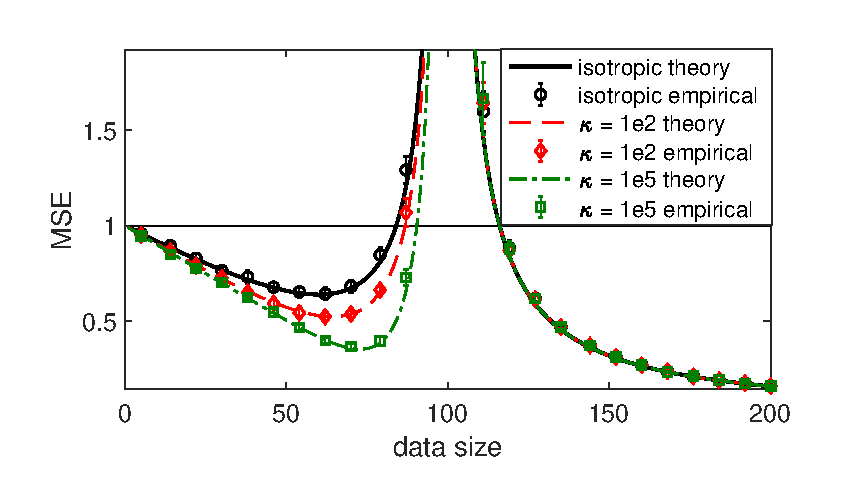
\includegraphics[width=0.6\textwidth]{figs/descent-intro-nice}
  \end{center}
  \begin{theorem}[Asymptotic consistency]
    Under previous assumptions,
    if additionally
    $\mu$ is sub-Gaussian with parameter uniformly bounded
    for all $d$,
    then
    \begin{align*}
      \underbrace{\MSE{\X^\dagger\y}}_{\text{i.i.d.}}\ -\ \underbrace{\MSE{\Xb^\dagger\ybb}}_{\text{surrogate}}\  \to\ 0
    \end{align*}
    with probability one as $d,n \to \infty$ with $n/d \to \bar c \in (0,\infty) \setminus \{1\}$.
  \end{theorem}
  
\end{frame}

\begin{frame}
  \frametitle{Main result II: Implicit ridge regularization}
  Why does ``Modern'' ML work?\\
  Because it induces implicit regularization
  % \footnote{Mahoney (2012).~arXiv:1203.0786}
  % \footnote{Neyshabur, Tomioka, Srebro (2014).~arXiv:1412.6614}
  \\[10mm]

   \textbf{Our contribution:}\\
  Implicit \textit{ridge} regularization of the
  minimum-norm interpolating model $\X^\dagger\y$
  \vspace{5mm}

  \begin{theorem}
For surrogate design $\Xb\sim S_{\mu}^n$ with $n<d$, we have:
    \vspace{-4mm}
    \begin{align*}
    \E[\Xb^\dagger\ybb]
     & \,=\,
    \argmin_\w\E\big[(\x^\top\w-y)^2\big] + \overbrace{\lambda
    \,\|\w\|^2}^{\text{ridge}}               
  \end{align*}
  where $\lambda$ is defined so that
  \[\underbrace{\text{sample size}}_{n}
    \ =\ \underbrace{\text{$\lambda$-effective dimension}}_{\tr((\Sigmab_\mu+\lambda\I)^{-1}\Sigmab_\mu)}\]
\end{theorem}
  
  % Same surrogate design also shows implicit regularization in
  % sketched optimizations
  % \footnote{Derezi\'{n}ski, Liang, Liao, Mahoney (2020) NeurIPS}

\end{frame}

\begin{frame}
  \frametitle{Consistency of implicit ridge regularization}
  \begin{center}
    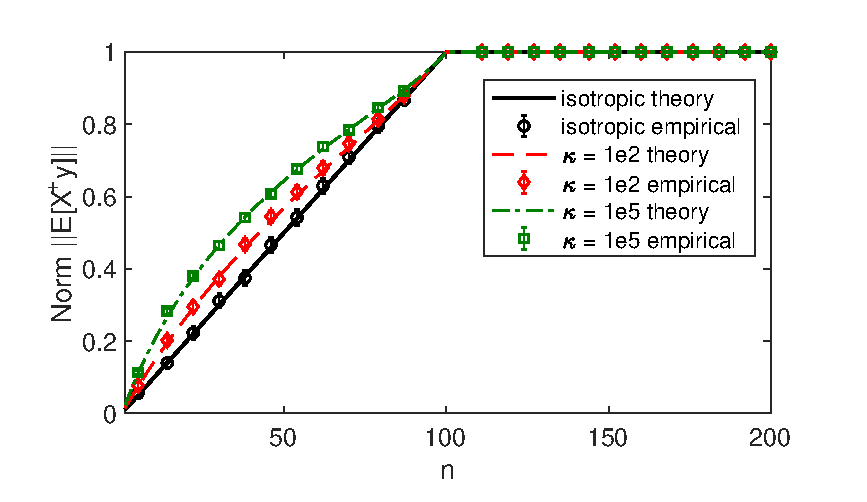
\includegraphics[width=0.6\textwidth]{figs/descent-shrinkage}
  \end{center}

\textbf{General phenomenon:} implicit regularization of random projections [DLLM20]
 
\begin{align*}
\E\big[ \!\!\! \underbrace{\I-\X^\dagger\X}_{\text{residual projection}}\!\!\big]\
\overset\epsilon\approx\ (\tfrac1{\lambda}\Sigmab_{\mu}+\I)^{-1}
  \quad\text{for }\X\sim\mu^n,\quad n<d.
\end{align*}
In [DLLM20], we show that if $\X\sim\mu^n$ is sub-Gaussian, then $\epsilon = O\Big(\frac1{\sqrt{\text{stable rank of }\Sigmab_{\mu}}}\Big)$.
  
%   Follow-up work: 
% \textrm{\textit{``Precise expressions for random projections: Low-rank
%   approximation and randomized Newton''}}, by Micha{\l} Derezi\'nski,
% Feynman Liang, Zhenyu Liao, Michael Mahoney

\let\thefootnote\relax\footnotetext{\hspace{-5mm}
\normalsize  [DLLM20]
\textit{``Precise expressions for random projections: Low-rank
  approximation and randomized Newton''}, at NeurIPS'20.}

  % \begin{theorem}[Asymptotic consistency]
  %   Under previous assumptions,
  %   if additionally
  %   $\mu$ is sub-Gaussian with parameter uniformly bounded
  %   for all $d$,
  %   then
  %   \begin{align*}
  %     \underbrace{\MSE{\X^\dagger\y}}_{\text{i.i.d.}}\ -\ \underbrace{\MSE{\Xb^\dagger\ybb}}_{\text{surrogate}}\  \to\ 0
  %   \end{align*}
  %   with probability one as $d,n \to \infty$ with $n/d \to \bar c \in (0,\infty) \setminus \{1\}$.
  % \end{theorem}
  
\end{frame}


% \begin{frame}
%   \frametitle{Surrogate random designs}

%   \textbf{Original problem}:
%   $\X \sim \mu^n$ has i.i.d.\ rows $\x_i^\top \sim \mu$

%   \textbf{Key trick}:
%   Consider surrogate $\tilde{\X} \sim S_\mu^n$,
%   tractable to analyze in overparameterized $n < d$ case,
%   equivalent as $n,d \to \infty$.

%   \pause

%   \begin{definition}[Surrogate design] \label{d:surrogate}
%     $\tilde{\X} \sim S_\mu^n$ is a random variable with same
%     support as $\X\sim\mu^K$ such that~for any
%     event $E$ measurable w.r.t.~$\X$, we have\vspace{-2mm}
%     \begin{align*}
%       \Pr\big\{\Xb\in E\big\}\ = \frac{\E[\pdet(\X\X^\top)\one_{[\X\in E]}]}{\E[\pdet(\X\X^\top)]}.
%     \end{align*}
%     Here, $\pdet(\cdot)$ denotes the pseudo-determinant, and
%     $K$ is a truncated Poisson random variable $\Poisson(\gamma_n)$ with
%     $\gamma_n$ chosen so that the sample size $\#(\Xb)$ satisfies $\E[\#(\Xb)]=n$.
%   \end{definition}
% \end{frame}

% \begin{frame}
%   \frametitle{Key properties of surrogate design}

%   \begin{lemma}[Lemma 2]\label{l:proj}
%     If  $\Xb\sim S_\mu^n$ and $n<d$, then we have:
%     $\E\big[\I-\Xb^\dagger\Xb\big] = (\gamma_n\Sigmab_\mu+\I)^{-1}$.
%   \end{lemma}

%   \begin{lemma}[Lemma 3]\label{l:sqinv-all}
%     If  $\Xb\sim S_\mu^n$ and $n<d$, then:
%     $\E\big[\tr\big((\Xb^\top\Xb)^{\dagger}\big)\big]
%       =\gamma_n\big(1-
%       \det\!\big((\tfrac1{\gamma_n}\I+\Sigmab_\mu)^{-1}\Sigmab_\mu\big)\big)$.
%   \end{lemma}

%   Double-descent result follows from applying above to bias-variance decomposition.

%   \pause

%   \begin{lemma}[Lemma 12]\label{l:ridge-over}
%     If $\Xb\sim S_\mu^n$ and $n>d$, then for any real-valued random function $y(\cdot)$
%     such that $\E_{\mu,y}[y(\x)\,\x]$ is well-defined,
%     denoting $\yb_i$ as $y(\xbb_i)$, we have
%     \begin{align*}
%       \E\big[\Xb^\dagger \ybb\big]
%        & =\Sigmab_\mu^{-1}\E_{\mu,y}\big[y(\x)\,\x\big].
%     \end{align*}
%   \end{lemma}

%   Implicit regularization result (as well as lemma 2) follow from specific choices of $y(\x)$.
% \end{frame}

% \begin{frame}
%   \frametitle{Asymptotic equivalence}

%   How does $\tilde{\X} \sim S_\mu^n$
%   compare to $\X \sim \mu^n$ (as $n,d \to \infty$)?
%   \pause
%   \begin{lemma}[Lemma 1]
%     If $\tilde{\X} \sim S_\mu^n$, then
%     $\E[ \text{\#rows}(\tilde{\X})] = n$
%   \end{lemma}
%   \pause
%   \begin{theorem}[Theorem 3]
%     Under previous assumptions,
%     if additionally
%     $\mu$ is sub-Gaussian with parameter uniformly bounded
%     for all $d$,
%     then
%     \begin{align*}
%       \MSE{\X^\dagger\y} - \Mc(\Sigmab, \w^*,\sigma^2,n) \to 0
%     \end{align*}
%     with probability one as $d,n \to \infty$ with $n/d \to \bar c \in (0,\infty) \setminus \{1\}$.
%   \end{theorem}
% \end{frame}

% \begin{frame}
%   \frametitle{Experiments verifying asymptotic equivalence}

%   \begin{center}
%     \hspace{-.8cm}
%     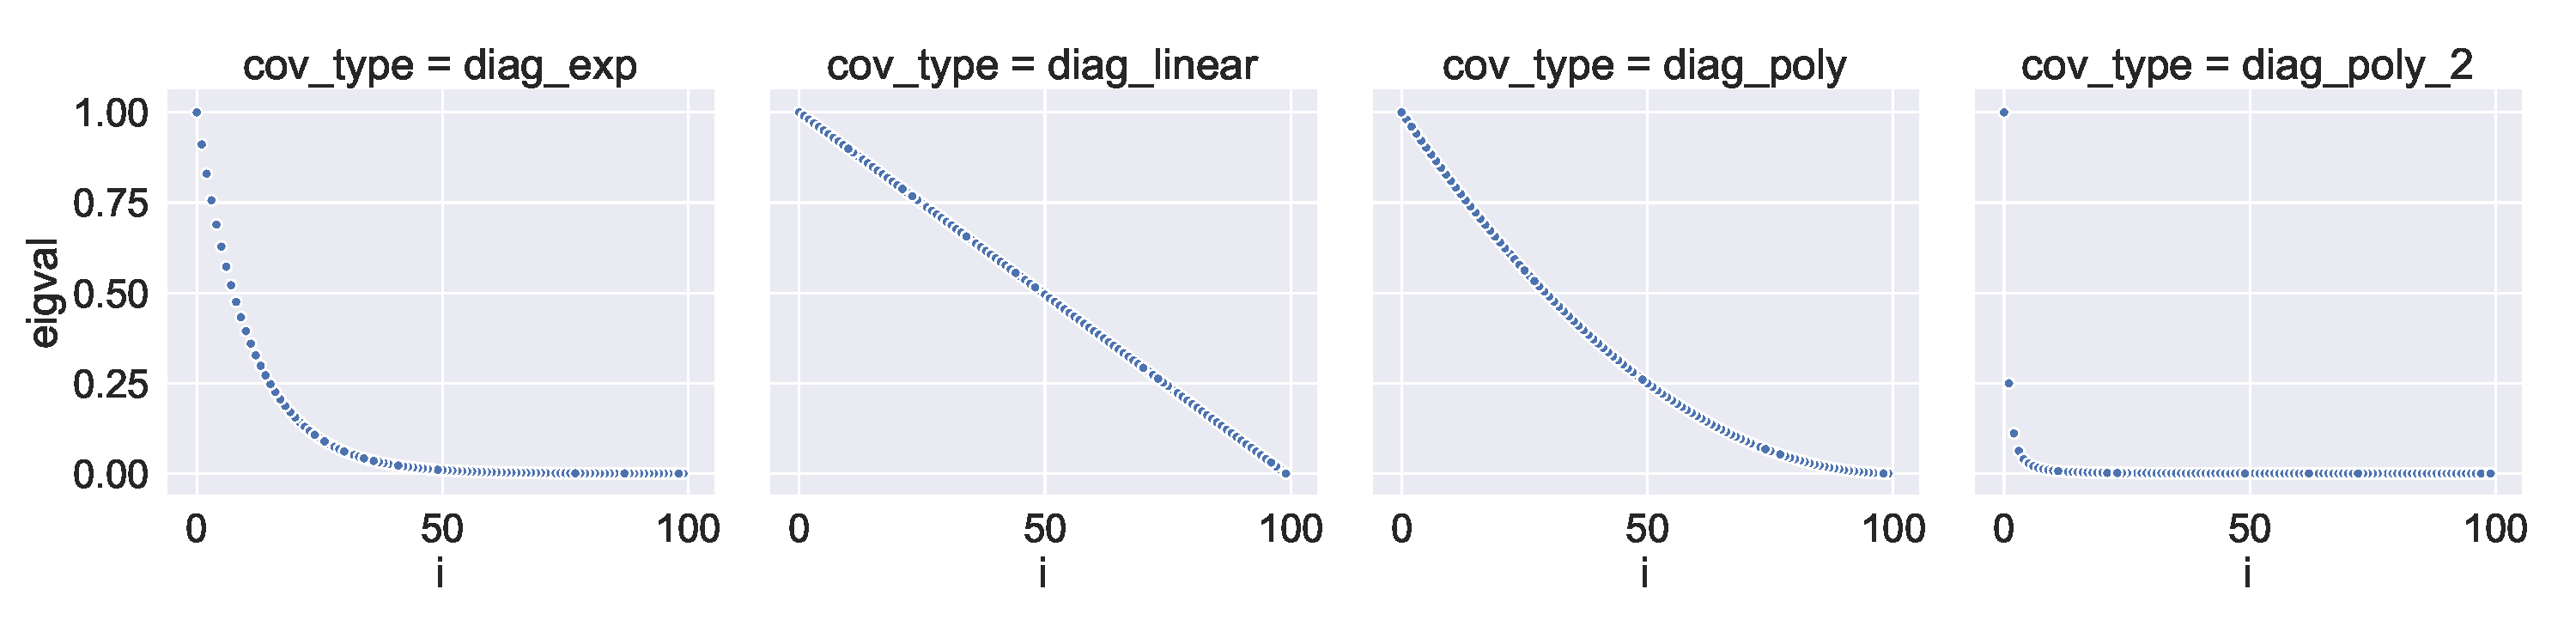
\includegraphics[width=0.93\textwidth]{continuous_figures/decays.pdf}
%     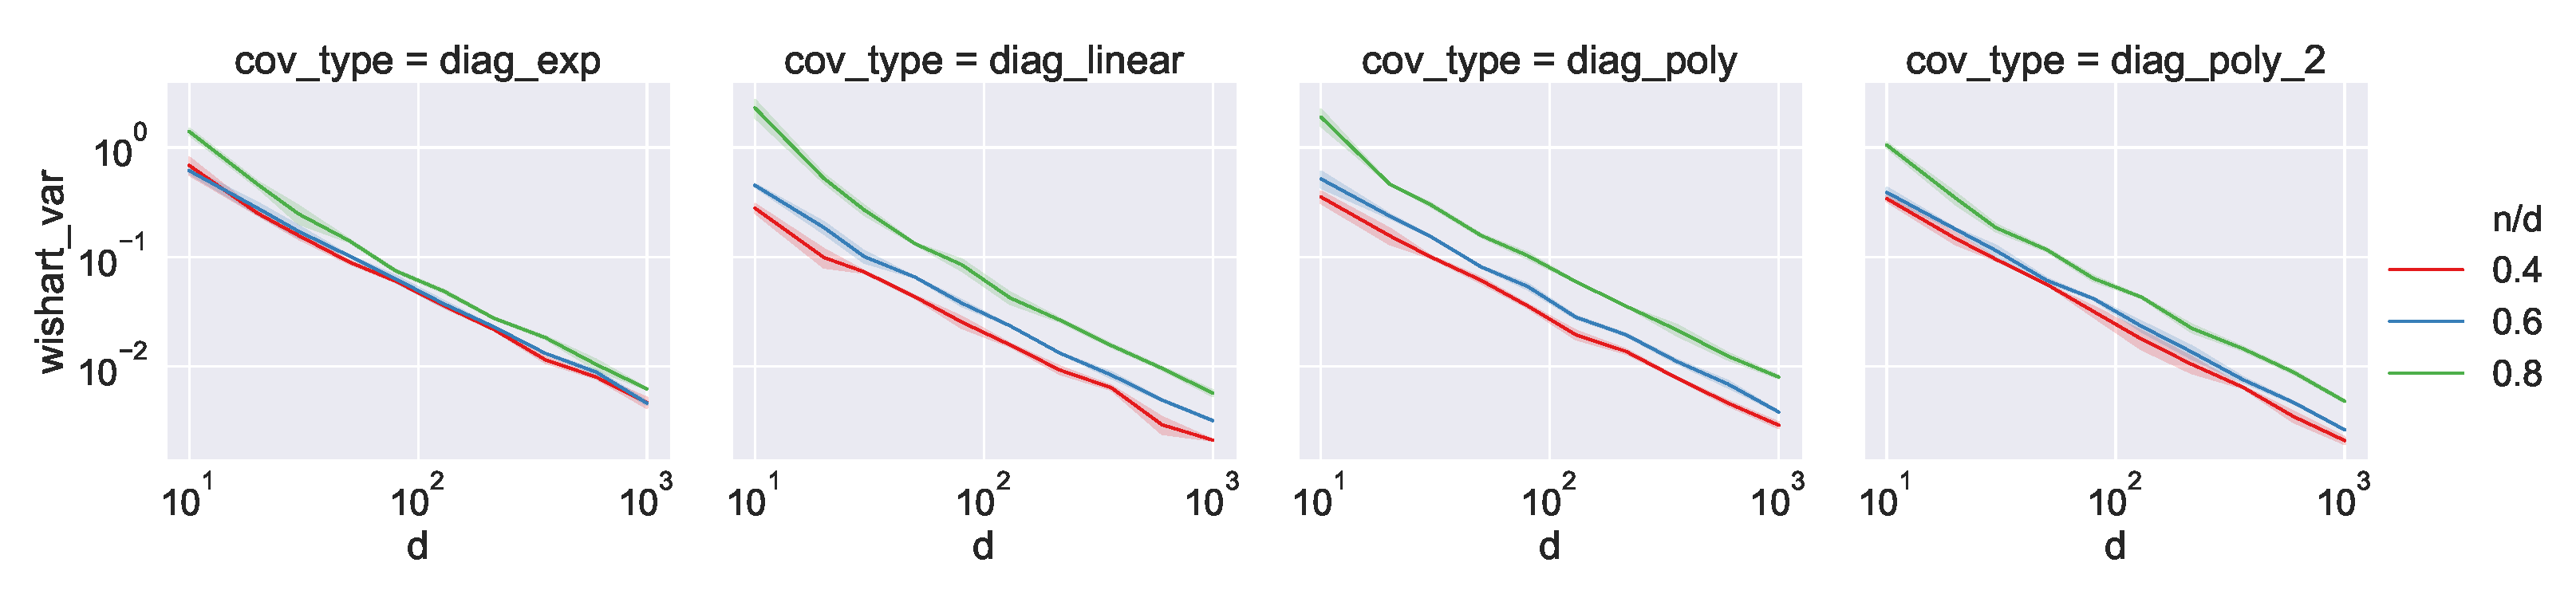
\includegraphics[width=\textwidth]{continuous_figures/wishart_var.pdf}
%     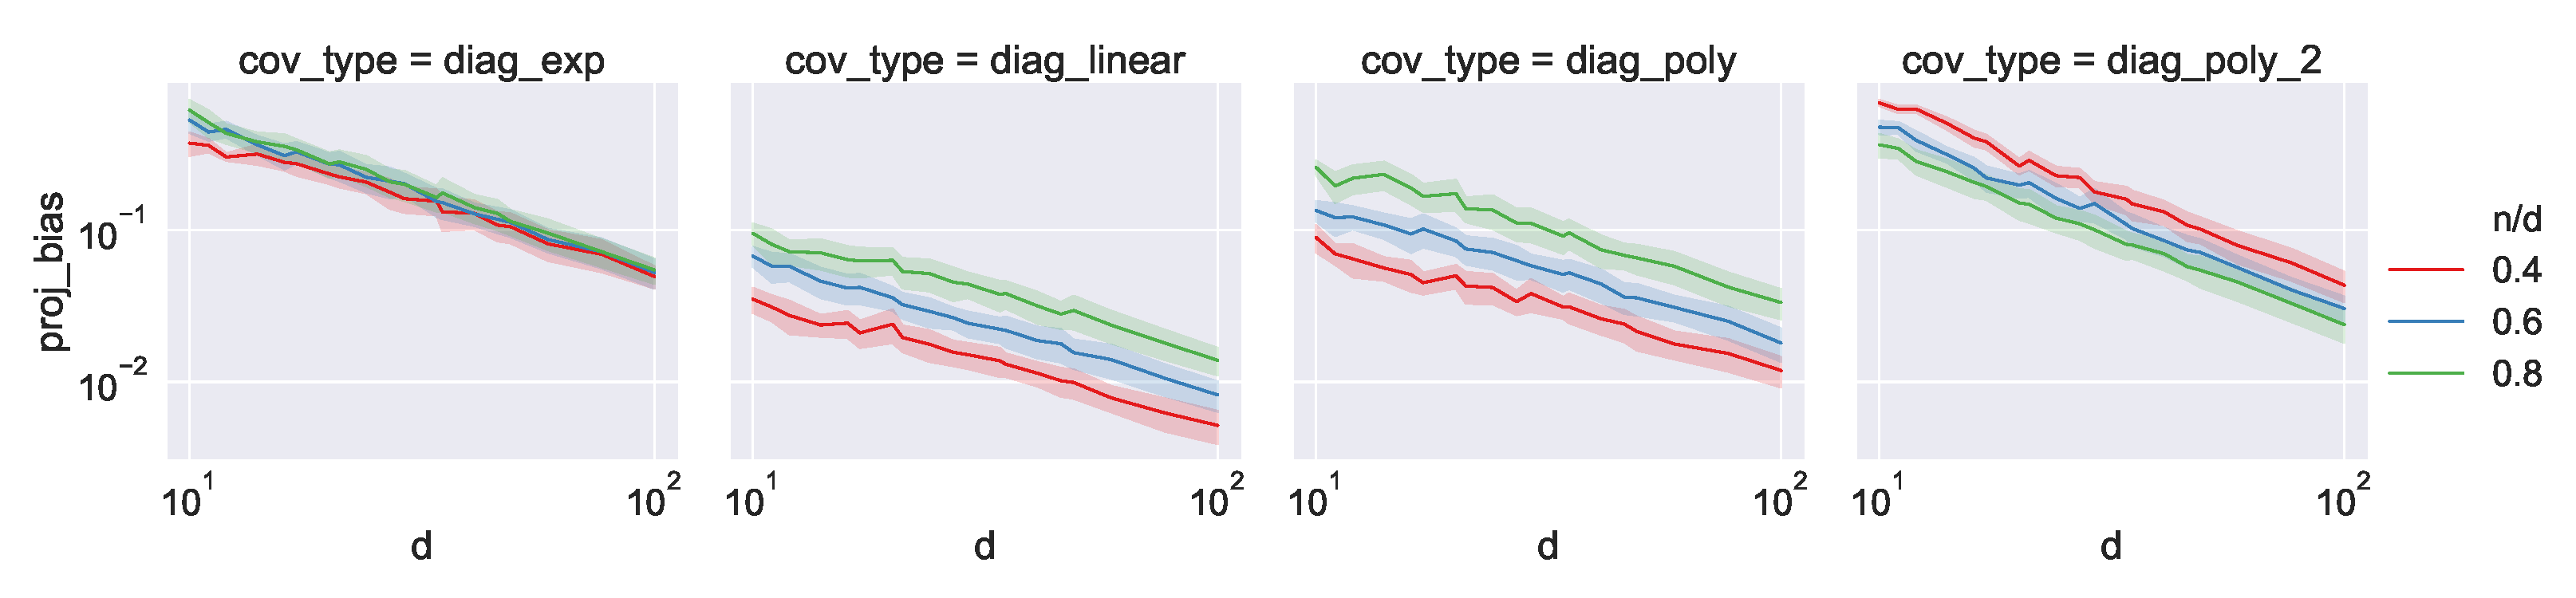
\includegraphics[width=\textwidth]{continuous_figures/proj_bias.pdf}
%   \end{center}
% \end{frame}


\end{document}
